%!TEX root = main.tex


\section{Introduction}

Games play a central role in AI research. In the early $20^{th}$ century, \cite{zermelo1913} showed that perfect information games in extensive form can be solved by a bottom-up traversal of the game tree. Despite the fact that this does not readily provide efficient ways to solve large games such as Chess or Go in practice, this has indeed 
laid the foundation for the dramatic progress in the field of perfect information games, with computer programs being able to challenge human experts. Solving games becomes more intricate when the players (agents) have incomplete information about the state of the game -- Poker for instance, where a player does not know the cards of the others. One of the remarkable imperfect information games where computer programs have been able to defeat professional human players is Texas Hold'em Poker~\cite{libratus-poker,deepstack,pluribus-poker}. A main technique used in these algorithms is the abstraction of large games into smaller \emph{imperfect recall} games. 

Perfect recall is the ability of a player to remember her own actions. Poker is an imperfect information game played by several players. However, ideally one would assume that the players have a perfect recall of their actions. An imperfect recall player does not remember the sequence of her own actions. Imperfect recall allows for a structured mechanism to forget the information history and as \cite{ijcai2024p332} argues, it is particularly suited for AI agents.

From a modeling perspective, imperfect recall has been used to describe teams of agents, where each team can be represented as a single agent with imperfect recall~\cite{VONSTENGEL1997309,DBLP:conf/aaai/Celli018} or to describe agents modeling multiple nodes which do not share information between each other due to privacy reasons~\cite{DBLP:conf/aaai/Conitzer19}. Moreover~\cite{LAMBERT2019164} argues that imperfect recall is a model of bounded rationality. Given the limited memory of players, it is not realistic to assume that the players remember all their actions. We refer the reader to~\cite{ijcai2024p332} for an excellent introduction to different uses of imperfect recall.  
From a practical perspective, the most prominent use of imperfect recall is in abstracting games~\cite{PracticalUseImperfect,DBLP:conf/aaai/GanzfriedS14,DBLP:conf/atal/BrownGS15, CERMAK2020103248}. The state space generated by usual games is typically very large and abstractions are crucial for solving such games. Abstractions that preserve perfect recall force a player to distinguish the current information gained, in all later rounds, even if it is not relevant. Abstractions using players with imperfect recall have been shown to outperform those using players with perfect recall~\cite{ DBLP:conf/sara/WaughZJKSB09, johanson2013evaluating, DBLP:conf/atal/BrownGS15,DBLP:conf/ijcai/CermakBL17}.



From a complexity perspective, imperfect recall games are known to be $\NP$-hard

~\cite{KollerMegiddo::1992,Cermak::2018} even when there is a single player, whereas perfect recall games can be solved in polynomial-time~\cite{KollerMegiddo::1992,vonStengel::1996}. Recent studies have aligned the complexity of different solution concepts for imperfect recall games to the modern complexity classes~\cite{GPS20,tewolde-et-al:2023,ijcai2024p332}. The hardness of imperfect recall games has motivated the search for subclasses which are polynomial-time solvable~\cite{kline2002minimum,kaneko1995behavior}, or where algorithms similar to the perfect recall case can be applied~\cite{DBLP:conf/icml/LanctotGBB12,DBLP:conf/sigecom/KroerS16}. The class of \emph{A-loss recall}~\cite{kline2002minimum,kaneko1995behavior} is a special kind of imperfect recall, where the loss of information can be traced back to a player forgetting her own action at a point in the past -- the player remembers \emph{where} it was played, but forgets \emph{what} was played. We consider A-loss recall games to be \emph{simple} since there are polynomial-time algorithms for solving them. To the best of our knowledge, A-loss recall games are the biggest known class of imperfect recall with a polynomial-time solution. This has led to research towards finding A-loss recall abstractions~\cite{Cermak::2018}. 

\emph{Contributions.} Our broad goal in this work is to find efficient ways to solve imperfect recall games in extensive-form. We do so by simplifying them into A-loss recall games. We focus on games where the players are not absent-minded: a player is absent-minded if she even forgets whether a decision point was previously seen or not. Here are our major contributions.
\begin{enumerate}\item We first identify a class of one-player games where the player's information structure is more complex than A-loss recall, but shuffling the order of actions results in an equivalent A-loss recall game. This leads to a new $\mathsf{PTIME}$ solvable class of imperfect recall games, that extends A-loss recall (\cref{thm:1p-shuffle-ptime}, \cref{cor:effic-solv-class}, \cref{cor:2-effic-solv-class}). Furthermore, these classes themselves can be tested in $\mathsf{PTIME}$. 

\item We show that every game with \emph{non-absentminded} players can be transformed into an equivalent A-loss recall game (\cref{thm:existence-alr-span}). We present an algorithm to generate an equivalent A-loss recall game with the smallest size.
\end{enumerate}
















 


The caveat in the second result above is that the resulting A-loss recall game could be exponentially bigger. This is expected, since solving imperfect recall games is $\NP$-hard, whereas A-loss recall games can be solved in polynomial-time. The result however shows that in order to solve imperfect recall games, one could either use a worst-case exponential-time algorithm on the original game, or apply our transformation to a worst-case exponential-sized game and run a polynomial-time algorithm on it. From a conceptual point of view, our result shows that as long as there is no absentmindedness, imperfect recall can be transformed into one where the information loss can be attributed to forgetting own actions at a past point.


\emph{Organization of the document.} Section~\ref{sec:an-example} introduces a modification of the popular matching pennies game that will be used as a running example to illustrate our results. Section~\ref{sec:background} recalls necessary preliminaries on extensive-form games. Section~\ref{sec:shuffled-loss-recall} presents the new polynomial-time class of shuffled A-loss recall. Section~\ref{sec:span} generalizes the idea of shuffling to incorporate a ``linear combination'' of action sequences, and presents the second result mentioned above. Section~\ref{sec:two-player} extends the results to the two-player setting. 

  






  



\section{An example}
\label{sec:an-example}



Let us start with a one-player game called the \emph{single team matching-unmatching pennies game}, which will be used as a running example. A team of players with the same goal can be interpreted as a single player. 
In this case, the team consists of two players Alice and Bob, each possessing a coin with two sides, Head (H) and Tail (T) and each of them must choose a side for their respective coins independently. 
The game unfolds in the following manner : a fair $n$-faced die with outcomes from $\{0, \dots, n-1 \}$ is rolled; then Alice chooses a side from $\{H,T\}$, followed by Bob choosing from $\{H,T\}$. Winning or losing depends on the parity of the die outcome. If the outcome of the die is even, then they win if and only if they match their sides. If the outcome is odd, they win if and only if their sides do not match. We consider three variants depending on what Alice and Bob can observe, and model it in extensive form in \cref{fig:match-penny-3-die} for $n=3$. An informal description of the figures follows after this paragraph.
\begin{description}
  \item[I.] Both Alice and Bob observe nothing (\cref{fig:match-penny-3-die-a}).
  \item[II.] Alice can't distinguish between die outcome $2i$ and $2i+1$ for $i \geq 0$,  but Bob observes nothing (\cref{fig:match-penny-3-die-b}).
   \item[III.] Alice can't distinguish between die outcome $2i$ and $2i+1$ for $i \geq 0$, Bob only observes coin of Alice but not outcome of die (\cref{fig:match-penny-3-die-c}). 
 \end{description} 
Alice and Bob want to maximize their \emph{expected payoff}. We will see their possible strategies in Section~\ref{sec:background}.  
Later, we will see that game \textbf{I} falls under the simple class of A-loss recall. 
In Section~\ref{sec:shuffled-loss-recall} and \cref{sec:span} we will see how to simplify games \textbf{II} and \textbf{III} respectively. 
%!TEX root = ../main.tex

\begin{figure}

\begin{subfigure}{0.45\columnwidth}
\centering
\tikzset{
triangle/.style = {regular polygon,regular polygon sides=3,draw,inner sep = 2},
circ/.style = {circle,fill=cyan!10,draw,inner sep = 3},
term/.style = {circle,draw,inner sep = 1.5,fill=black},
sq/.style = {rectangle,fill=gray!20, draw, inner sep = 4}
}
\begin{tikzpicture}[scale=0.8]

\tikzstyle{level 1}=[level distance=18mm,sibling distance=24mm]
\tikzstyle{level 2}=[level distance=11mm,sibling distance=12mm]
\tikzstyle{level 3}=[level distance=11mm,sibling distance=5mm]

\begin{scope}[->, >=stealth]
 \node(0)[triangle]{}
    child{  
    node(00)[circ,draw=black]{}
        child{
        node(000)[circ]{}
            child{
            node(0000)[term,label=below:{\scriptsize $1$}]{} 
            edge from parent node[left,pos = 0.3,inner sep=1.5]{\scriptsize H}
            }
            child{
            node(0001)[term,label=below:{\scriptsize $0$}]{}
            edge from parent node[right,pos = 0.3,inner sep=1.5]{\scriptsize T}                
            }
        edge from parent node[left,pos = 0.2]{{\scriptsize H}}                
        }
        child{
        node(001)[circ]{}
            child{
            node(0010)[term,label=below:{\scriptsize $0$}]{} 
            edge from parent node[left,pos = 0.3,inner sep=1.5]{\scriptsize H}
            }
            child{
            node(0011)[term,label=below:{\scriptsize $1$}]{}
            edge from parent node[right,pos = 0.3,inner sep=1.5]{\scriptsize T}                
            }
        edge from parent node[right,pos = 0.2]{{\scriptsize T}}
        }
    edge from parent node[above,pos = 0.8]{0}
    edge from parent node[above,pos = 0.4]{\scriptsize $\frac{1}{3}$} 
    }
    child{
    node(01)[circ]{}
        child{
        node(010)[circ]{}
            child{
            node(0100)[term,label=below:{\scriptsize $0$}]{}
            edge from parent node[left,pos = 0.3,inner sep=1.5]{\scriptsize H}
            }
            child{
            node(0101)[term,label=below:{\scriptsize $1$}]{}
            edge from parent node[right,pos = 0.3,inner sep=1.5]{\scriptsize T}                
            }
        edge from parent node[left,pos = 0.2]{\scriptsize H}
        }
        child{
        node(011)[circ]{}
            child{
            node(0110)[term,label=below:{\scriptsize $1$}]{} 
            edge from parent node[left,pos = 0.3,inner sep=1.5]{\scriptsize H}
            }
            child{
            node(0111)[term,label=below:{\scriptsize $0$}]{}
            edge from parent node[right,pos = 0.3,inner sep=1.5]{\scriptsize T}                
            } 
        edge from parent node[right,pos = 0.2]{\scriptsize T}
        }
    edge from parent node[right,pos = 0.8]{1}
    edge from parent node[left,pos = 0.4]{\scriptsize $\frac{1}{3}$}
    }
    child{
    node(02)[circ]{}
        child{
        node(020)[circ]{}
            child{
            node(0200)[term,label=below:{\scriptsize $1$}]{}
            edge from parent node[left,pos = 0.3,inner sep=1.5]{\scriptsize H}
            }
            child{
            node(0201)[term,label=below:{\scriptsize $0$}]{}
            edge from parent node[right,pos = 0.3,inner sep=1.5]{\scriptsize T}                
            }
        edge from parent node[left,pos = 0.2]{\scriptsize H}
        }
        child{
        node(021)[circ]{}
            child{
            node(0210)[term,label=below:{\scriptsize $0$}]{} 
            edge from parent node[left,pos = 0.3,inner sep=1.5]{\scriptsize H}
            }
            child{
            node(0211)[term,label=below:{\scriptsize $1$}]{}
            edge from parent node[right,pos = 0.3,inner sep=1.5]{\scriptsize T}                
            } 
        edge from parent node[right,pos = 0.2]{\scriptsize T}
        }
    edge from parent node[above,pos = 0.8]{2}
    edge from parent node[above,pos = 0.4]{\scriptsize $\frac{1}{3}$}
    }
    ;

\end{scope}
\draw [dashed,thick,blue,out=22,in=158] (00) to (01); 
\draw [dashed,thick,blue,out=22,in=158] (01) to (02); 
\draw [dashed,ForestGreen,thick,out=22,in=158] (001) to (010);
\draw [dashed,ForestGreen,thick,out=22,in=158] (000) to (001);
\draw [dashed,ForestGreen,thick,out=22,in=158] (010) to (011);
\draw [dashed,ForestGreen,thick,out=22,in=158] (011) to (020);
\draw [dashed,ForestGreen,thick,out=22,in=158] (020) to (021);

%\node[fit=(1),dashed,thick,blue, draw, circle,inner sep=1pt] {};


%\node[fit=(2),dashed,thick,black, draw, circle,inner sep=1pt] {};

\end{tikzpicture}
\caption{Alice and Bob, both observe nothing}
\label{fig:match-penny-3-die-a}
\end{subfigure}
\vspace{6mm}
\begin{subfigure}{0.48\columnwidth}
\centering
\tikzset{
triangle/.style = {regular polygon,regular polygon sides=3,draw,inner sep = 2},
circ/.style = {circle,fill=cyan!10,draw,inner sep = 3},
term/.style = {circle,draw,inner sep = 1.5,fill=black},
sq/.style = {rectangle,fill=gray!20, draw, inner sep = 4}
}
\begin{tikzpicture}[scale=0.8]

\tikzstyle{level 1}=[level distance=18mm,sibling distance=24mm]
\tikzstyle{level 2}=[level distance=11mm,sibling distance=12mm]
\tikzstyle{level 3}=[level distance=11mm,sibling distance=5mm]

\begin{scope}[->, >=stealth]
 \node(0)[triangle]{}
    child{  
    node(00)[circ,draw=black]{}
        child{
        node(000)[circ]{}
            child{
            node(0000)[term,label=below:{\scriptsize $1$}]{} 
            edge from parent node[left,pos = 0.3,inner sep=1.5]{\scriptsize H}
            }
            child{
            node(0001)[term,label=below:{\scriptsize $0$}]{}
            edge from parent node[right,pos = 0.3,inner sep=1.5]{\scriptsize T}                
            }
        edge from parent node[left,pos = 0.2]{{\scriptsize H}}                
        }
        child{
        node(001)[circ]{}
            child{
            node(0010)[term,label=below:{\scriptsize $0$}]{} 
            edge from parent node[left,pos = 0.3,inner sep=1.5]{\scriptsize H}
            }
            child{
            node(0011)[term,label=below:{\scriptsize $1$}]{}
            edge from parent node[right,pos = 0.3,inner sep=1.5]{\scriptsize T}                
            }
        edge from parent node[right,pos = 0.2]{{\scriptsize T}}
        }
    edge from parent node[above,pos = 0.8]{0} 
    edge from parent node[above,pos = 0.4]{\scriptsize $\frac{1}{3}$}
    }
    child{
    node(01)[circ]{}
        child{
        node(010)[circ]{}
            child{
            node(0100)[term,label=below:{\scriptsize $0$}]{}
            edge from parent node[left,pos = 0.3,inner sep=1.5]{\scriptsize H}
            }
            child{
            node(0101)[term,label=below:{\scriptsize $1$}]{}
            edge from parent node[right,pos = 0.3,inner sep=1.5]{\scriptsize T}                
            }
        edge from parent node[left,pos = 0.2]{\scriptsize H}
        }
        child{
        node(011)[circ]{}
            child{
            node(0110)[term,label=below:{\scriptsize $1$}]{} 
            edge from parent node[left,pos = 0.3,inner sep=1.5]{\scriptsize H}
            }
            child{
            node(0111)[term,label=below:{\scriptsize $0$}]{}
            edge from parent node[right,pos = 0.3,inner sep=1.5]{\scriptsize T}                
            } 
        edge from parent node[right,pos = 0.2]{\scriptsize T}
        }
    edge from parent node[right,pos = 0.8]{1}
    edge from parent node[left,pos = 0.4]{\scriptsize $\frac{1}{3}$}
    }
    child{
    node(02)[circ]{}
        child{
        node(020)[circ]{}
            child{
            node(0200)[term,label=below:{\scriptsize $1$}]{}
            edge from parent node[left,pos = 0.3,inner sep=1.5]{\scriptsize H}
            }
            child{
            node(0201)[term,label=below:{\scriptsize $0$}]{}
            edge from parent node[right,pos = 0.3,inner sep=1.5]{\scriptsize T}                
            }
        edge from parent node[left,pos = 0.2]{\scriptsize H}
        }
        child{
        node(021)[circ]{}
            child{
            node(0210)[term,label=below:{\scriptsize $0$}]{} 
            edge from parent node[left,pos = 0.3,inner sep=1.5]{\scriptsize H}
            }
            child{
            node(0211)[term,label=below:{\scriptsize $1$}]{}
            edge from parent node[right,pos = 0.3,inner sep=1.5]{\scriptsize T}                
            } 
        edge from parent node[right,pos = 0.2]{\scriptsize T}
        }
    edge from parent node[above,pos = 0.8]{2}
    edge from parent node[above,pos = 0.4]{\scriptsize $\frac{1}{3}$}
    }
    ;

\end{scope}
\node[fit=(02),dashed,thick,red, draw, circle,inner sep=1pt] {};
\draw [dashed,thick,blue,out=22,in=158] (00) to (01); 
\draw [dashed,ForestGreen,thick,out=22,in=158] (001) to (010);
\draw [dashed,ForestGreen,thick,out=22,in=158] (000) to (001);
\draw [dashed,ForestGreen,thick,out=22,in=158] (010) to (011);
\draw [dashed,ForestGreen,thick,out=22,in=158] (011) to (020);
\draw [dashed,ForestGreen,thick,out=22,in=158] (020) to (021);
%\node[fit=(1),dashed,thick,blue, draw, circle,inner sep=1pt] {};


%\node[fit=(2),dashed,thick,black, draw, circle,inner sep=1pt] {};

\end{tikzpicture}
\caption{Alice can't distinguish between $2i$ and $2i+1$ for $i \geq 0$, Bob observes nothing}
\label{fig:match-penny-3-die-b}
\end{subfigure}

\begin{subfigure}{\columnwidth}
\centering
\tikzset{
triangle/.style = {regular polygon,regular polygon sides=3,draw,inner sep = 2},
circ/.style = {circle,fill=cyan!10,draw,inner sep = 3},
term/.style = {circle,draw,inner sep = 1.5,fill=black},
sq/.style = {rectangle,fill=gray!20, draw, inner sep = 4}
}
\begin{tikzpicture}[scale=0.8]

\tikzstyle{level 1}=[level distance=18mm,sibling distance=24mm]
\tikzstyle{level 2}=[level distance=11mm,sibling distance=12mm]
\tikzstyle{level 3}=[level distance=11mm,sibling distance=5mm]

\begin{scope}[->, >=stealth]
 \node(0)[triangle]{}
    child{  
    node(00)[circ,draw=black]{}
        child{
        node(000)[circ]{}
            child{
        node(0000)[term,label=below:{\scriptsize $1$}]{} 
            edge from parent node[left,pos = 0.2]{\scriptsize H}
            }
            child{
            node(0001)[term,label=below:{\scriptsize $0$}]{}
            edge from parent node[right,pos = 0.2]{\scriptsize T}                
            }
        edge from parent node[left,pos = 0.2]{{\scriptsize H}}                
        }
        child{
        node(001)[circ]{}
            child{
            node(0010)[term,label=below:{\scriptsize $0$}]{} 
            edge from parent node[left,pos = 0.2]{\scriptsize H}
            }
            child{
            node(0011)[term,label=below:{\scriptsize $1$}]{}
            edge from parent node[right,pos = 0.2]{\scriptsize T}                
            }
        edge from parent node[right,pos = 0.2]{{\scriptsize T}}
        }
    edge from parent node[above,pos = 0.8]{0} 
    edge from parent node[above,pos = 0.4]{\scriptsize $\frac{1}{3}$}
    }
    child{
    node(01)[circ]{}
        child{
        node(010)[circ]{}
            child{
            node(0100)[term,label=below:{\scriptsize $0$}]{}
            edge from parent node[left,pos = 0.2]{\scriptsize H}
            }
            child{
            node(0101)[term,label=below:{\scriptsize $1$}]{}
            edge from parent node[right,pos = 0.2]{\scriptsize T}                
            }
        edge from parent node[left,pos = 0.2]{\scriptsize H}
        }
        child{
        node(011)[circ]{}
            child{
            node(0110)[term,label=below:{\scriptsize $1$}]{} 
            edge from parent node[left,pos = 0.2]{\scriptsize H}
            }
            child{
            node(0111)[term,label=below:{\scriptsize $0$}]{}
            edge from parent node[right,pos = 0.2]{\scriptsize T}                
            } 
        edge from parent node[right,pos = 0.2]{\scriptsize T}
        }
    edge from parent node[right,pos = 0.8]{1}
    edge from parent node[left,pos = 0.4]{\scriptsize $\frac{1}{3}$}
    }
    child{
    node(02)[circ]{}
        child{
        node(020)[circ]{}
            child{
            node(0200)[term,label=below:{\scriptsize $1$}]{}
            edge from parent node[left,pos = 0.2]{\scriptsize H}
            }
            child{
            node(0201)[term,label=below:{\scriptsize $0$}]{}
            edge from parent node[right,pos = 0.2]{\scriptsize T}                
            }
        edge from parent node[left,pos = 0.2]{\scriptsize H}
        }
        child{
        node(021)[circ]{}
            child{
            node(0210)[term,label=below:{\scriptsize $0$}]{} 
            edge from parent node[left,pos = 0.2]{\scriptsize H}
            }
            child{
            node(0211)[term,label=below:{\scriptsize $1$}]{}
            edge from parent node[right,pos = 0.2]{\scriptsize T}                
            } 
        edge from parent node[right,pos = 0.2]{\scriptsize T}
        }
    edge from parent node[above,pos = 0.8]{2}
    edge from parent node[above,pos = 0.4]{\scriptsize $\frac{1}{3}$}
    }
    ;

\end{scope}
\node[fit=(02),dashed,thick,red, draw, circle,inner sep=1pt] {};
\draw [dashed,thick,blue,out=22,in=158] (00) to (01);
\draw [dashed,thick,ForestGreen,out=28,in=152] (000) to (010);
\draw [dashed,ForestGreen,thick,out=28,in=152] (010) to (020);
\draw [dashed,brown,thick,out=28,in=152] (001) to (011);
\draw [dashed,brown,thick,out=28,in=152] (011) to (021);
%\node[fit=(1),dashed,thick,blue, draw, circle,inner sep=1pt] {};


%\node[fit=(2),dashed,thick,black, draw, circle,inner sep=1pt] {};

\end{tikzpicture}
\caption{Bob only observes Alice's coin}
\label{fig:match-penny-3-die-c}
\end{subfigure}


% \begin{subfigure}{.48\columnwidth}
% \centering
% \tikzset{
% triangle/.style = {regular polygon,regular polygon sides=3,draw,inner sep = 2},
% circ/.style = {circle,fill=cyan!10,draw,inner sep = 3},
% term/.style = {circle,draw,inner sep = 1.5,fill=black},
% sq/.style = {rectangle,fill=gray!20, draw, inner sep = 4}
% }
% \begin{tikzpicture}[scale=0.8]

% \tikzstyle{level 1}=[level distance=15mm,sibling distance=23mm]
% \tikzstyle{level 2}=[level distance=10mm,sibling distance=12mm]
% \tikzstyle{level 3}=[level distance=12mm,sibling distance=4mm]

% \begin{scope}[->, >=stealth]
%  \node(0)[triangle]{}
%     child{  
%     node(00)[circ,draw=black]{}
%         child{
%         node(000)[circ]{}
%             child{
%             node(0000)[term,label=below:{\scriptsize $1$}]{} 
%             edge from parent node[left,pos = 0.2]{\scriptsize H}
%             }
%             child{
%             node(0001)[term,label=below:{\scriptsize $0$}]{}
%             edge from parent node[right,pos = 0.2]{\scriptsize T}                
%             }
%         edge from parent node[left,pos = 0.2]{{\scriptsize H}}                
%         }
%         child{
%         node(001)[circ]{}
%             child{
%             node(0010)[term,label=below:{\scriptsize $0$}]{} 
%             edge from parent node[left,pos = 0.2]{\scriptsize H}
%             }
%             child{
%             node(0011)[term,label=below:{\scriptsize $1$}]{}
%             edge from parent node[right,pos = 0.2]{\scriptsize T}                
%             }
%         edge from parent node[right,pos = 0.2]{{\scriptsize T}}
%         }
%     edge from parent node[above,pos = 0.8]{0} 
%     }
%     child{
%     node(01)[circ]{}
%         child{
%         node(010)[circ]{}
%             child{
%             node(0100)[term,label=below:{\scriptsize $0$}]{}
%             edge from parent node[left,pos = 0.2]{\scriptsize H}
%             }
%             child{
%             node(0101)[term,label=below:{\scriptsize $1$}]{}
%             edge from parent node[right,pos = 0.2]{\scriptsize T}                
%             }
%         edge from parent node[left,pos = 0.2]{\scriptsize H}
%         }
%         child{
%         node(011)[circ]{}
%             child{
%             node(0110)[term,label=below:{\scriptsize $1$}]{} 
%             edge from parent node[left,pos = 0.2]{\scriptsize H}
%             }
%             child{
%             node(0111)[term,label=below:{\scriptsize $0$}]{}
%             edge from parent node[right,pos = 0.2]{\scriptsize T}                
%             } 
%         edge from parent node[right,pos = 0.2]{\scriptsize T}
%         }
%     edge from parent node[right,pos = 0.8]{1}
%     }
%     child{
%     node(02)[circ]{}
%         child{
%         node(020)[circ]{}
%             child{
%             node(0200)[term,label=below:{\scriptsize $1$}]{}
%             edge from parent node[left,pos = 0.2]{\scriptsize H}
%             }
%             child{
%             node(0201)[term,label=below:{\scriptsize $0$}]{}
%             edge from parent node[right,pos = 0.2]{\scriptsize T}                
%             }
%         edge from parent node[left,pos = 0.2]{\scriptsize H}
%         }
%         child{
%         node(021)[circ]{}
%             child{
%             node(0210)[term,label=below:{\scriptsize $0$}]{} 
%             edge from parent node[left,pos = 0.2]{\scriptsize H}
%             }
%             child{
%             node(0211)[term,label=below:{\scriptsize $1$}]{}
%             edge from parent node[right,pos = 0.2]{\scriptsize T}                
%             } 
%         edge from parent node[right,pos = 0.2]{\scriptsize T}
%         }
%     edge from parent node[above,pos = 0.8]{2}
%     }
%     ;

% \end{scope}
% \draw [dashed,thick,blue,out=22,in=158] (00) to (01); 
% \draw [dashed,ForestGreen,thick,out=22,in=158] (000) to (021);
% \draw [dashed,brown,thick,out=22,in=158] (001) to (011);
% \draw [dashed,brown,thick,out=22,in=158] (010) to (020);
% %\node[fit=(1),dashed,thick,blue, draw, circle,inner sep=1pt] {};


% %\node[fit=(2),dashed,thick,black, draw, circle,inner sep=1pt] {};

% \end{tikzpicture}
% \caption{Bob can't distinguish between $(i,\text{C})$ and $(i+1 \mod n,\text{C})$ for $i \geq 0 $, $C \in \{H,T\}$ and $n=3$}
% \label{fig:match-penny-3-die-d}
% \end{subfigure}

\caption{Three versions of the single team matching-unmatching pennies game for $n=3$}
\label{fig:match-penny-3-die}
\end{figure}

Before we delve into the background and results, here is a description of the extensive-form model. 
The root node, marked with a triangle, is the event of rolling the die. The triangle nodes are called $\chance$ nodes, and the
edges out of them associate probabilities to each of the outcomes. For this game, the distribution is uniform. The circle nodes denote decision nodes of the team. The nodes in the second level (root being the first level) belong to Alice whereas the nodes in the third level belong to Bob. The actions labelled in edges out of these nodes denote the actions available to the corresponding players. 
A leaf node indicates an end state, and a path from root to leaf denotes
a play from start to end. The number associated with a leaf gives the
payoff that the team receives at the end of the corresponding play. E.g., in \cref{fig:match-penny-3-die-a} in the play resulting from the path $0, H, T$ the payoff is $0$ because the team loses. It is $1$ when they win. 

Imperfect information is expressed using a dotted line: a player cannot distinguish between two nodes joined by a dotted line.
For e.g., in \cref{fig:match-penny-3-die-a} the dotted red line joining all of Alice's nodes indicates that Alice cannot observe the die outcome. Similarly, the blue dotted line for Bob indicates, he neither observes the outcome of the die, nor the side of the coin chosen by Alice. These sets of indistinguishable nodes are called \emph{information sets}.





\section{Background and notations}
\label{sec:background}

%!TEX root = ../main.tex

\begin{figure}
%\begin{center}
\tikzset{
triangle/.style = {regular polygon,regular polygon sides=3,draw,inner sep = 2},
circ/.style = {circle,fill=cyan!10,draw,inner sep = 3},
term/.style = {circle,draw,inner sep = 1.5,fill=black},
sq/.style = {rectangle,fill=gray!20, draw, inner sep = 4}
}

\begin{subfigure}{.45\columnwidth}
\centering
\begin{tikzpicture}[scale=0.9]
\tikzstyle{level 1}=[level distance=9mm,sibling distance = 22mm]
\tikzstyle{level 2}=[level distance=7mm,sibling distance=10mm]
\tikzstyle{level 3}=[level distance=7mm,sibling distance=6mm]
\tikzstyle{level 4}=[level distance=7mm,sibling distance=5mm]

%node (ij) is the j th node in i th level

\begin{scope}[->, >=stealth]
\node (0) [circ] {}
child {
  node (00) [triangle] {}
  child {
    node (000) [circ] {}
    child {
      node (0000) [term, label=below:{}] {}
      edge from parent node [left] {\scriptsize $c$}
    }
    child {
      node (0001) [term, label=below:{}] {}
      edge from parent node [right] {\scriptsize $d$}
      }
    edge from parent node [left] {}
  }
  child {
    node (001) [circ] {}
    child {
      node (0010) [term, label=below:{}] {}
      edge from parent node [left] {\scriptsize $c$}
    }
    child {
      node (0011) [term, label=below:{}] {}
      edge from parent node [right] {\scriptsize $d$}
      }
    edge from parent node [right] {} 
  }
  edge from parent node [above] {\scriptsize$a$}
}
child {
  node (01) [triangle] {}
   child {
     node (010) [circ] {}
     child {
      node (0100) [term, label=below:{}] {}
      edge from parent node [left] {\scriptsize $e$}
    }
    child {
      node (0101) [term, label=below:{}] {}
      edge from parent node [right] {\scriptsize $f$}
      }
    edge from parent node [left] {}
  }
  child {
    node (011) [circ] {}
    child {
      node (0110) [term, label=below:{}] {}
      edge from parent node [left] {\scriptsize $e$}
    }
    child {
      node (0111) [term, label=below:{}] {}
      edge from parent node [right] {\scriptsize $f$}
      }
    edge from parent node [right] {} 
  }
  edge from parent node [above] {\scriptsize$b$}
}
;
\end{scope}

%observations
%\draw [dashed, thick, red, in=150,out=30](00) to (01) ;

  \node[fit=(0),dashed,thick,red, draw, circle,inner sep=1pt] {};
\draw [dashed, thick, blue, in=150,out=30] (000) to (001) ;
\draw [dashed, thick, ForestGreen, in=150,out=30] (010) to (011);

%node labels
\node [black] at (0,0.35) {\scriptsize $r$};
\node [black] at (-1,-0.55) {\scriptsize $u_1$};
\node [black] at (1, -0.55) {\scriptsize $u_2$};
\node [black] at (-2, -1.5) {\scriptsize $u_3$};
\node [black] at (-.25, -1.5) {\scriptsize $u_4$};

\node [black] at (0.25, -1.5) {\scriptsize $u_5$};
\node [black] at (2, -1.5) {\scriptsize $u_6$};

%obs labels
\node [red] at (0,-.5) {\scriptsize $I_1$};
\node [blue] at (-1.1,-1.6) {\scriptsize $I_2$};
\node [ForestGreen] at (1.1,-1.6) {\scriptsize $I_3$};



\end{tikzpicture}

\caption{$\Max$ with perfect recall}
\label{fig-allexmp-pftrec}
\end{subfigure}
\quad
\begin{subfigure}{.45\columnwidth}
\centering
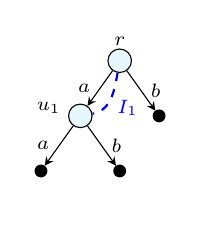
\begin{tikzpicture}
\tikzstyle{level 1}=[level distance=7mm,sibling distance = 10mm]
\tikzstyle{level 2}=[level distance=7mm,sibling distance=10mm]
\tikzstyle{level 3}=[level distance=7mm,sibling distance=15mm]
\tikzstyle{level 4}=[level distance=7mm,sibling distance=8mm]

%\draw [help lines, step=0.5] (-3,-3) grid (3,0);

\begin{scope}[->, >=stealth]
\node (0) [circ] {}
child{
  node (1) [circ] {}
  child{
    node (3) [term, label=below:{}] {}
    edge from parent node [left] {\scriptsize $a$}
  }
  child{
    node (4) [term,label=below:{}] {}
    edge from parent node [right] {\scriptsize $b$}
  }
  edge from parent node [left] {\scriptsize $a$}
}
child{
  node (2) [term, label=below:{}] {}
  edge from parent node [right] {\scriptsize $b$}
}
;
\end{scope}

\draw [dashed, thick, blue, in=10,out=-100] (0) to (1);



\node [black] at (0,0.25) {\scriptsize $r$};
\node [black] at (-.9,-0.6) {\scriptsize $u_1$};



\node [blue] at (.1,-.6) {\scriptsize $I_1$};

\end{tikzpicture}
\caption{$\Max$ with absentmindedness}
\label{fig-allexmp-absentm}
\end{subfigure}


%\end{center}
\caption{Recalls of $\Max$}
\label{fig:recall-examples}
\end{figure}

This section presents the formal definitions. The single team matching-unmatching pennies game has only one player and chance nodes, but in general we will talk about zero-sum two player games. As in \cref{fig:2-p-shuffle}, there are two players $\Max$ (circle nodes) and $\Min$ (square nodes). The payoff at the leaf, is the amount $\Min$ loses and $\Max$ gains. The goal of $\Max$ is to maximize the expected payoff whereas $\Min$ wishes to minimize it. In \cref{fig:match-penny-3-die} $\Max$ was the team consisting of Alice and Bob.







In this paper, we mainly work with \emph{game-structures} and not games
themselves. Game-structures are essentially games sans the numerical
quantities. Any game on a game structure can be represented symbolically as in shown \cref{fig:alossSpan-a} with symbolic payoffs $z_i$s and symbolic chance probabilities $p_i$s (with constraints on $p_i$'s). An extensive
form game can be obtained from a game structure by plugging in values for $z_i$s and $p_i$s.  We work with game structures because the
notions of perfect recall and imperfect recall can be determined
simply by looking at the game-structure.


Formally, a game-structure $\Tt$ is a tuple $(V, L, r, A, E, \Ii)$
where $V$ is a finite set of non-terminal nodes partitioned as
$V_{\Max}$, $V_{\Min}$ and $V_{\chance}$; $L$ is a finite set of leaves;
$r \in V$ is a root node; $A = A_{\Max} \cup A_{\Min}$ is a finite set
of actions; $E \incl V \times (V \cup L)$ is an edge
relation that induces a directed tree; edges originating from $V_{\Max} \cup V_{\Min}$ are labelled with actions from $A$; we write $u \xra{a} v$ if
$(u, v)$ is labelled with $a$, and assume that there is no incoming edge
$u \xra{} r$ to the root node $r$; $\Ii = \Ii_{\Max} \cup \Ii_{\Min}$
is a set of information sets for $i \in \{ \Max, \Min \}$, each
information set $I \in \Ii_i$ is a subset of vertices belonging to
$i$, i.e. $I \incl V_i$, and moreover, the set of information sets
$\Ii_i$ partitions $V_i$. E.g., in \cref{fig-allexmp-pftrec},
$\Ii_{\Max} = \{I_1, I_2, I_3\}$ and $I_1 = \{r\}, I_2 = \{u_3, u_4\}$
and $I_3 = \{u_5, u_6\}$. We can understand these information sets as a signal that the player receives when she reaches a node in it. On receiving the signal, the player knows the actions that are available to play at that position. 

An information set models the fact that a player cannot distinguish
between the nodes within it. Therefore, the set of outgoing actions
from each node in an information set is required to be the same. This
allows us to define $\act(I)$ as the set of actions available at
information set $I$. E.g., in \cref{fig-allexmp-pftrec},
$\act(I_2) = \{c, d\}$. For technical convenience, we make a second
assumption: for all $I, I' \in \Ii$ with $I \neq I'$, we have
$\act(I) \cap \act(I') = \emptyset$. Therefore, the actions identify
the information sets. With this assumption, in \cref{fig:match-penny-3-die}, the actions of Alice should be seen as $H_A, T_A$ and those of Bob's as $H_B, T_B$. But we omit the subscripts in the figure for clarity. 
\begin{definition}[Extensive form games]\label{def:ext-form-games}
  A two-player zero-sum game in extensive form is a tuple
  $(\Tt,\d, \Uu)$ where $\Tt$ is a game-structure, $\d$ is the
  \emph{chance probability} associating to each $\chance$ node, a
  probability distribution on the outgoing actions, and
  $\Uu : L \mapsto \Rat $ is the utility function associating a payoff
  to each leaf.
\end{definition}

The \emph{size} of a game is the sum of the bit-lengths of all chance probabilities and leaf
payoffs in it. A \emph{behavioral strategy} for player $\Max$ ($\Min$ resp.) assigns a probability
distribution to $\act(I)$ for each $I \in \Ii_{\Max}$ ($\Ii_{\Min}$ resp.). Once we fix behavioral strategies $\sigma$ and $\tau$ for $\Max$ and $\Min$ respectively,
each edge in the game has an associated probability of being taken,
given by the corresponding strategy or $\chance$. The probability of reaching a leaf $u \in L$ is given by the product of all the numbers along the path to the leaf. Consider \cref{fig:shuffle-a}.
Let $\sigma$ assign $\frac{1}{4}$ to $b$ and $\frac{3}{4}$ to
$\bar{b}$; $0$ and $1$ to $c$ and $\bar{c}$, and $\frac{1}{3}$ to $a$
and $\frac{2}{3}$ to $\bar{a}$. The probability of reaching the leaf $b \bar{a}$ is 
then: $p_1 \times \frac{1}{4} \times \frac{2}{3}$. For a leaf $u$, we denote this quantity by
$\prob_{\sigma, \tau}(u)$. The \emph{expected payoff} $\Ee(\s, \t)$
when $\Max$ plays $\sigma$ and $\Min$ plays $\tau$, then equals
$\sum_{u \in L} \prob_{\s, \t} (u) \Uu(u)$. The solution concept that we
will consider in this paper is the notion of maxmin.
The \emph{maxmin value} of a game is the
following: \[\max\limits_{\s}\min\limits_{\t}\Ee(\s,\t)\] where
$\s,\t$ are behavioral strategies of $\Max$ and $\Min$ respectively. A
strategy of $\Max$ which provides the maxmin value is called a
\emph{maxmin strategy}. In one-player games, we only have $\Max$ player and the maxmin value of the game is $\max\limits_{\s}\Ee(\s)$. For one-player non-absentminded games, the maxmin value can be in fact obtained by a \emph{pure strategy} -- pure strategies are special cases of behavioural strategies which assign either $0$ or $1$ to each action~\cite{KollerMegiddo::1992}.

The maxmin value of the game in \cref{fig:match-penny-3-die-a} is $\frac{2}{3}$ since Alice and Bob can win at most in 2 of the 3 die rolls by playing matching sides. Another way to see this is to consider the four possible pure strategies $HH, HT, TH, TT$, which induce payoffs $\frac{2}{3}$, $\frac{1}{3}$, $\frac{1}{3}$ and $\frac{2}{3}$ respectively. Now since, in the rest of the following two versions, the team has more information \footnote{This can be observed by the fact that information sets in each version are refinements of the previous versions.} they can guarantee at least $\frac{2}{3}$ by playing the same strategy. Interestingly, one can observe (by enumerating all pure strategies) that they cannot do better than that in any version. 
\paragraph*{Histories and recalls.} We now move on to describing the
various types of imperfect information, based on what the player
remembers about her history. A node $w \in V$ is reached by a unique
path from the root: $r = v_0 \xra{} v_1 \xra{} \cdots \xra{} v_n =
w$. Let $v_{i_1}, v_{i_2}, \dots, v_{i_k}$ be the vertices in this
sequence which do not belong to $\chance$. Then,
$\his(w) = a_{1} a_{2} \cdots a_{k-1}$, where $v_{i_j} \xra{a_j} v_{i_{j + 1}}$.
For a player $i \in \{\Max, \Min\}$ the history of $i$ at $w$, denoted
by $\his_i(w)$, is the sequence of player $i$'s actions in the path to
$w$, which is simply the sub-sequence of $\his(w)$ restricted to
actions from $A_i$. E.g.: in \cref{fig-allexmp-pftrec},
$\his_{\Max}(u_3) = \his_{\Max}(u_4) = a$; in
\cref{fig:shuffle-a}, $\his_{\Max}(u_3) = b$ and $\his_{\Max}(u_2) = \epsilon$, the empty sequence. It is important to remark that this definition uses the assumption that actions determine information sets -- otherwise, we would need to incorporate the information sets that were visited along the way, into the history.



Let $\Hh$ denote the set of all histories and $\Hh_i$ be the set of
all histories of player $i$. For an information set $I \in \Ii_i$ let
$\Hh(I) = \{ \his(u) \mid u \in I\}$ be the set of histories of all
nodes in $I$. Similarly, we can define $\Hh_i(I)$ with respect to
$\Hh_i$. Let $\Hh(L)$ denote the set of all leaf histories.
When $\Hh_i(I)$ has multiple histories, at a node $v \in I$ the player
does not remember which history she traversed to reach $v$. Hence the
player loses information. For two
nodes $u$ and $v$ in $I$, comparing $\his_i(u)$ and $\his_i(v)$
reveals the loss or retention of previously withheld information at
the respective nodes. To capture this there are different notions of
\emph{recall}.

\emph{Perfect recall.} Player $i$ is said to have \emph{perfect
  recall} ($\pfr$) if for every $I \in \Ii_i$, and every pair of
distinct vertices $u, v \in I$, we have $\his_i(u) = \his_i(v)$,
i.e. $|\Hh_i(I)| = 1$.  Otherwise, the player is said to have imperfect
recall.  \cref{fig-allexmp-pftrec} is an example of a perfect recall
game.
\emph{Imperfect recall.} \cref{fig:shuffle-a} gives an example of
a game-structure that has imperfect recall. Notice that states $u_3$
and $u_4$ lie in the same information set $I_3$, but the sequence of
the player's actions leading to these states is different: history at
$u_3$ is $b$, whereas at $u_4$ it is $\bar{b}$. 
Within imperfect recall,
there are distinctions. The imperfect recall in
~\cref{fig:shuffle-b} and the one in ~\cref{fig:shuffle-a}
are in some sense different: in ~\cref{fig:shuffle-b}, the
inability to distinguish between the two nodes in $I_1$ can be traced back to
a point in the past where she forgets her own action from some
information set ($I_3$ in this case), whereas in \cref{fig:shuffle-a}, the player has been able to
distinguish between the two outcomes of the $\chance$ node, but later
forgets at $I_3$ where she started from, leading to four histories $b,\bar{b},c$ and $\bar{c}$ at $I_3$.


\emph{A-loss recall.} Game-structures as in \cref{fig:shuffle-b} are said to have \emph{A-loss
  recall}. A consequence of having A-loss recall is that a player always remembers any new information
gained from $\chance$ outcomes, which is not the case
in~\cref{fig:shuffle-a}. Player $i$ has \emph{A-loss recall}
($\alr$) if for all $I \in \Ii_i$, and every pair of distinct vertices
$u, v \in I$, either $\his_i(u) = \his_i(v)$, or $\his_i(u)$ is of the
form $s a s_1$, and $\his_i(v)$ of the form $s b s_2$, where
$a, b \in \act(I')$ for some $I' \in \Ii$, with $a \neq b$. The game in \cref{fig:match-penny-3-die-a} has A-loss recall, whereas the others, \cref{fig:match-penny-3-die-b} and \cref{fig:match-penny-3-die-c} do not.  

Finally, player $i$ is said to be
\emph{non-absentminded} ($\nam$) if $\forall u, v \in V_i$ with $u$
lying on the path to $v$, the information set that $u$ belongs to is
different from the information set that $v$ belongs
to, i.e. all nodes of $i$ on a path from $r$ to leaf node lie in distinct
information sets. \cref{fig-allexmp-absentm} is an example where
$\Max$ is absentminded, since both $r$ and $u_1$ lie in the same
information set. Notice that $\pfr$ implies $\alr$, which in turn implies implies $\nam$. 

When $\Max$ and $\Min$ have recalls $R_{\Max}, R_{\Min} \in \{ $\pfr$,~$\alr$,~$\nam$ \} $
respectively we will denote the game as a
$(R_{\Max}, R_{\Min})$-game. A one-player game with recall $R$ is denoted as $R$-game. In this paper we are only concerned with one-player $\nam$-games and two-player $(\nam,\nam)$-games. Let us now recall some known
results.
\begin{itemize}\item A maxmin solution in a $(\pfr,\alr)$-game can be computed in
  polynomial- time~\\\cite{KollerMegiddo::1992,vonStengel::1996,kaneko1995behavior}. As a corollary, an optimal solution in a one-player $\alr$-game can be computed in
  polynomial-time ~\cite{kaneko1995behavior}.

\item The maxmin decision problem for $(\nam,\nam)$-games is both
  $\NP$-hard~\cite{KollerMegiddo::1992} and

  
  $\sqsum$-hard~\cite{GPS20} \footnote{$\sqsum$ is the decision problem of checking
    if the sum of the square roots of $k$ positive integers is less
    than another positive number}.
   The $\NP$-hardness and the $\sqsum$-hardness hold even for
  $(\alr,\pfr)$-games~\cite{Cermak::2018,GPS20}. The maxmin decision problem for one-player $\nam$-games is
  $\NP$-complete~\cite{KollerMegiddo::1992}.
\end{itemize}


Our core idea is to view game structures through the polynomials they generate. 
\paragraph*{Leaf monomials.} In a game structure, assigning variable $x_a$ to each action
$a$, the monomial obtained by taking the product of all $x_a$ along the path to each leaf $t$ is called
a \emph{leaf monomial}, and denoted as $\mu(t)$. E.g., the leaf
monomials of the game-structure in \cref{fig-allexmp-pftrec} are
$\{ x_ax_c, x_ax_d, x_bx_e, x_bx_f\}$. For a game structure $\Tt$, we will write $X(\Tt)$ for the set of leaf monomials. For a game $G$, let
$\prob_{\chance}(t)$ denote the product of $\chance$ probabilities in
the path to $t$. The polynomial given by
$\sum\limits_{t \in L} \prob_{\chance}(t) \cdot \Uu(t) \cdot \mu(t)$
is called the \emph{payoff polynomial} of a game. 
A constraint of the form $\sum\limits_{a \in \act(I)} x_a = 1$ for an
information set $I$ will be called a \emph{strategy constraint}. Any non-negative valuation satisfying these constraints gives a behavioral strategy to the players.
The maxmin value in a game can be given by the maxmin of the payoff polynomial over all possible values satisfying the strategy constraints.


\paragraph*{Overview of our work}
In this work, our mantra for simplifying games is to find simpler games with same payoff polynomials (upto renaming of variables). Leaf monomials are the building blocks of payoff polynomials. We give methods to generate from a given game-structure $\Tt$, a transformed game-structure $\Tt'$ with A-loss recall such that: either $\Tt'$ has the same set of leaf monomials (Section~\ref{sec:shuffled-loss-recall}), or each leaf monomial of $\Tt$ is a linear combination of the leaf monomials of $\Tt'$ (Section~\ref{sec:span}).


\endinput



















%!TEX root = ../main.tex

\begin{figure}
\begin{subfigure}{0.5\columnwidth}
\centering
\tikzset{
triangle/.style = {regular polygon,regular polygon sides=3,draw,inner sep = 2},
circ/.style = {circle,fill=cyan!10,draw,inner sep = 3},
term/.style = {circle,draw,inner sep = 1.5,fill=black},
sq/.style = {rectangle,fill=gray!20, draw, inner sep = 4}
}

\begin{tikzpicture}[scale=0.85]
\tikzstyle{level 1}=[level distance=9mm,sibling distance = 22mm]
\tikzstyle{level 2}=[level distance=7mm,sibling distance=10mm]
\tikzstyle{level 3}=[level distance=7mm,sibling distance=6mm]
\tikzstyle{level 4}=[level distance=7mm,sibling distance=5mm]

%node (ij) is the j th node in i th level

\begin{scope}[->, >=stealth]
\node (0) [triangle] {}
child {
  node (00) [circ] {}
  child {
    node (000) [circ] {}
    child {
      node (0000) [term, label=below:{\scriptsize $z_1$}] {}
      edge from parent node [left] {\scriptsize $a$}
    }
    child {
      node (0001) [term, label=below:{\scriptsize $z_2$}] {}
      edge from parent node [right] {\scriptsize $\bar{a}$}
      }
    edge from parent node [left] {\scriptsize $b$}
  }
  child {
    node (001) [circ] {}
    child {
      node (0010) [term, label=below:{\scriptsize $z_3$}] {}
      edge from parent node [left] {\scriptsize $a$}
    }
    child {
      node (0011) [term, label=below:{\scriptsize $z_4$}] {}
      edge from parent node [right] {\scriptsize $\bar{a}$}
      }
    edge from parent node [right] {\scriptsize $\bar{b}$} 
  }
  edge from parent node [above] {\scriptsize $p_1$}
}
child {
  node (01) [circ] {}
   child {
     node (010) [circ] {}
     child {
      node (0100) [term, label=below:{\scriptsize $z_5$}] {}
      edge from parent node [left] {\scriptsize $a$}
    }
    child {
      node (0101) [term, label=below:{\scriptsize $z_6$}] {}
      edge from parent node [right] {\scriptsize $\bar{a}$}
      }
    edge from parent node [left] {\scriptsize $c$}
  }
  child {
    node (011) [circ] {}
    child {
      node (0110) [term, label=below:{\scriptsize $z_7$}] {}
      edge from parent node [left] {\scriptsize $a$}
    }
    child {
      node (0111) [term, label=below:{\scriptsize $z_8$}] {}
      edge from parent node [right] {\scriptsize $\bar{a}$}
      }
    edge from parent node [right] {\scriptsize $\bar{c}$} 
  }
  edge from parent node [above] {\scriptsize $p_2$}
}
;
 \node[fit=(00),dashed,thick,blue, draw, circle,inner sep=1pt] {};
  \node[fit=(01),dashed,thick,red, draw, circle,inner sep=1pt] {};
\end{scope}

\draw [dashed, thick, ForestGreen, in=150,out=30] (000) to (001);
\draw [dashed, thick, ForestGreen, in=150,out=30] (001) to (010);
\draw [dashed, thick, ForestGreen, in=150,out=30] (010) to (011);
%\draw [dashed, thick, blue, in=150,out=30] (000) to (001);
%\draw [dashed, thick, red, in=150,out=30] (010) to (011);

\node [black] at (0,0.35) {\scriptsize $r$};
\node [black] at (-1.5,-0.55) {\scriptsize $u_1$};
\node [black] at (1.5, -0.55) {\scriptsize $u_2$};
\node [black] at (-2, -1.6) {\scriptsize $u_3$};
\node [black] at (-.25, -1.7) {\scriptsize $u_4$};

\node [black] at (0.25, -1.7) {\scriptsize $u_5$};
\node [black] at (2, -1.6) {\scriptsize $u_6$};

%obs labels
\node [ForestGreen] at (0,-1.1) {\scriptsize $I_3$};
\node [blue] at (-.55,-.9) {\scriptsize $I_1$};
\node [red] at (.55,-.9) {\scriptsize $I_2$};

\end{tikzpicture}
\caption{$\Max$ without $\alr$ but has $\salr$}
\label{fig:shuffle-a}
\end{subfigure}
\begin{comment}
\begin{subfigure}{0.45\columnwidth}
%\centering
\tikzset{
triangle/.style = {regular polygon,regular polygon sides=3,draw,inner sep = 2},
circ/.style = {circle,fill=cyan!10,draw,inner sep = 3},
term/.style = {circle,draw,inner sep = 1.5,fill=black},
sq/.style = {rectangle,fill=gray!20, draw, inner sep = 4}
}

\begin{tikzpicture}[scale=0.85]
\tikzstyle{level 1}=[level distance=9mm,sibling distance = 22mm]
\tikzstyle{level 2}=[level distance=7mm,sibling distance=10mm]
\tikzstyle{level 3}=[level distance=7mm,sibling distance=6mm]
\tikzstyle{level 4}=[level distance=7mm,sibling distance=5mm]

%node (ij) is the j th node in i th level

\begin{scope}[->, >=stealth]
\node (0) [circ] {}
child {
  node (00) [triangle] {}
  child {
    node (000) [circ] {}
    child {
      node (0000) [term, label=below:{}] {}
      edge from parent node [left] {\scriptsize $b$}
    }
    child {
      node (0001) [term, label=below:{}] {}
      edge from parent node [right] {\scriptsize $\bar{b}$}
      }
    edge from parent node [left] {}
  }
  child {
    node (001) [circ] {}
    child {
      node (0010) [term, label=below:{}] {}
      edge from parent node [left] {\scriptsize $b$}
    }
    child {
      node (0011) [term, label=below:{}] {}
      edge from parent node [right] {\scriptsize $\bar{b}$}
      }
    edge from parent node [right] {} 
  }
  edge from parent node [above] {\scriptsize $a$}
}
child {
  node (01) [triangle] {}
   child {
     node (010) [circ] {}
     child {
      node (0100) [term, label=below:{}] {}
      edge from parent node [left] {\scriptsize $c$}
    }
    child {
      node (0101) [term, label=below:{}] {}
      edge from parent node [right] {\scriptsize $\bar{c}$}
      }
    edge from parent node [left] {}
  }
  child {
    node (011) [circ] {}
    child {
      node (0110) [term, label=below:{}] {}
      edge from parent node [left] {\scriptsize $c$}
    }
    child {
      node (0111) [term, label=below:{}] {}
      edge from parent node [right] {\scriptsize $\bar{c}$}
      }
    edge from parent node [right] {} 
  }
  edge from parent node [above] {\scriptsize $\bar{a}$}
}
;
\end{scope}

%\draw [dashed, thick, ForestGreen, in=150,out=30] (00) to (01);

\node[fit=(0),dashed,thick,ForestGreen, draw, circle,inner sep=1pt] {};
\draw [dashed, thick, blue, in=150,out=30] (000) to (010);
\draw [dashed, thick, red, in=150,out=30] (001) to (011);


\node [black] at (0,0.45) {\scriptsize $r$};
\node [black] at (-1.1,-0.45) {\scriptsize $u_1$};
\node [black] at (1.1, -0.45) {\scriptsize $u_2$};
\node [black] at (-2, -1.65) {\scriptsize $u_3$};
\node [black] at (-.2, -1.65) {\scriptsize $u_4$};

\node [black] at (0.25, -1.65) {\scriptsize $u_5$};
\node [black] at (2, -1.65) {\scriptsize $u_6$};

%obs labels
\node [ForestGreen] at (0,-0.6) {\scriptsize $I_3$};
\node [blue] at (-0.35,-1) {\scriptsize $I_1$};
\node [red] at (0.35,-1) {\scriptsize $I_2$};

\end{tikzpicture}
\caption{}
\label{fig:shuffle-c}
\end{subfigure}%
\end{comment}
\begin{subfigure}{0.48\columnwidth}
\centering
\tikzset{
triangle/.style = {regular polygon,regular polygon sides=3,draw,inner sep = 2},
circ/.style = {circle,fill=cyan!10,draw,inner sep = 3},
term/.style = {circle,draw,inner sep = 1.5,fill=black},
sq/.style = {rectangle,fill=gray!20, draw, inner sep = 4}
}

\begin{tikzpicture}[scale=0.85]
\tikzstyle{level 1}=[level distance=9mm,sibling distance = 22mm]
\tikzstyle{level 2}=[level distance=7mm,sibling distance=10mm]
\tikzstyle{level 3}=[level distance=7mm,sibling distance=6mm]
\tikzstyle{level 4}=[level distance=7mm,sibling distance=5mm]

%node (ij) is the j th node in i th level

\begin{scope}[->, >=stealth]
\node (0) [circ] {}
child {
  node (00) [triangle] {}
  child {
    node (000) [circ] {}
    child {
      node (0000) [term, label=below:{\scriptsize $z_1$}] {}
      edge from parent node [left] {\scriptsize $b$}
    }
    child {
      node (0001) [term, label=below:{\scriptsize $z_3$}] {}
      edge from parent node [right] {\scriptsize $\bar{b}$}
      }
    edge from parent node [left] {}
  }
  child {
    node (001) [circ] {}
    child {
      node (0010) [term, label=below:{\scriptsize $z_5$}] {}
      edge from parent node [left] {\scriptsize $c$}
    }
    child {
      node (0011) [term, label=below:{\scriptsize $z_7$}] {}
      edge from parent node [right] {\scriptsize $\bar{c}$}
      }
    edge from parent node [right] {} 
  }
  edge from parent node [above] {\scriptsize $a$}
}
child {
  node (01) [triangle] {}
   child {
     node (010) [circ] {}
     child {
      node (0100) [term, label=below:{\scriptsize $z_2$}] {}
      edge from parent node [left] {\scriptsize $b$}
    }
    child {
      node (0101) [term, label=below:{\scriptsize $z_4$}] {}
      edge from parent node [right] {\scriptsize $\bar{b}$}
      }
    edge from parent node [left] {}
  }
  child {
    node (011) [circ] {}
    child {
      node (0110) [term, label=below:{\scriptsize $z_6$}] {}
      edge from parent node [left] {\scriptsize $c$}
    }
    child {
      node (0111) [term, label=below:{\scriptsize $z_8$}] {}
      edge from parent node [right] {\scriptsize $\bar{c}$}
      }
    edge from parent node [right] {} 
  }
  edge from parent node [above] {\scriptsize $\bar{a}$}
}
;
\end{scope}

%\draw [dashed, thick, ForestGreen, in=150,out=30] (00) to (01);

\node[fit=(0),dashed,thick,ForestGreen, draw, circle,inner sep=1pt] {};
\draw [dashed, thick, blue, in=150,out=30] (000) to (010);
\draw [dashed, thick, red, in=150,out=30] (001) to (011);

%\node [black] at (0,0.45) {\scriptsize $r$};
%\node [black] at (-1.1,-0.45) {\scriptsize $u_1$};
%\node [black] at (1.1, -0.45) {\scriptsize $u_2$};
%\node [black] at (-2, -1.65) {\scriptsize $u_3$};
%\node [black] at (-.2, -1.65) {\scriptsize $u_4$};
%
%\node [black] at (0.25, -1.65) {\scriptsize $u_5$};
%\node [black] at (2, -1.65) {\scriptsize $u_6$};

%obs labels
\node [ForestGreen] at (0,-0.6) {\scriptsize $I_3$};
\node [blue] at (-0.35,-1) {\scriptsize $I_1$};
\node [red] at (0.35,-1) {\scriptsize $I_2$};

\node[black] at (-1.5,-.95) {\scriptsize $p_1$};
\node[black] at (-.73,-.95) {\scriptsize $p_2$};

\node[black] at (1.5,-.95) {\scriptsize $p_2$};
\node[black] at (.73,-.95) {\scriptsize $p_1$};
\end{tikzpicture}
\caption{$\Max$ with $\alr$}
\label{fig:shuffle-b}
\end{subfigure}
\caption{Equivalent $\alr$ game using $\salr$ for game without $\alr$ }
\label{fig:shuffle}
\end{figure}


\paragraph*{Shuffled A-loss recall}
The game-structure in \cref{fig:shuffle-a} does not have A-loss recall. This is because the player knows about $\chance$ outcomes $I_1$ and $I_2$ which she forgets at $I_3$.  Now, consider the game-structure in~\cref{fig:shuffle-c}, obtained by \emph{shuffling} the actions ($a$ goes above $b$ and $c$). This game-structure has A-loss recall. The crucial observation is that both the game-structures, \cref{fig:shuffle-a} and \cref{fig:shuffle-c}, lead to the same ``leaf monomials'': on assigning variable $x_a$ to an action labeled $a$, the product of the variables along the path to each leaf produces a leaf monomial. For instance, the leaf monomials for the game-structures in ~\cref{fig:shuffle-a} and ~\cref{fig:shuffle-c} respectively are $\{x_ax_b,x_ax_{\bar{b}},x_{\bar{a}}x_b,x_{\bar{a}}x_{\bar{b}},x_ax_c, x_ax_{\bar{c}},x_{\bar{a}}x_c,x_{\bar{a}}x_{\bar{c}} \}$.
We say that the game-structure of ~\cref{fig:shuffle-a} has \emph{shuffled A-loss recall}. Even though the game originally does not have A-loss recall, it can be shuffled in some way to get an A-recall structure. 
Not every game-structure has shuffled A-loss recall.

Our results:
\begin{itemize}
\item We provide a polynomial-time algorithm to identify whether a game-structure has shuffled A-loss recall. If the answer is yes, the algorithm also computes the shuffled game-structure.

\item As a result, we are able to show that one-player shuffled A-loss recall games can be solved in polynomial-time. Similarly, we deduce that two player games between a perfect recall player and a shuffled A-loss recall player can be solved in polynomial-time.
\end{itemize}






%!TEX root = ../main.tex

\begin{figure}
\centering

\begin{subfigure}{.3\columnwidth}
%\centering
\tikzset{
triangle/.style = {regular polygon,regular polygon sides=3,draw,inner sep = 2},
circ/.style = {circle,fill=cyan!10,draw,inner sep = 3},
term/.style = {circle,draw,inner sep = 1.5,fill=black},
sq/.style = {rectangle,fill=gray!20, draw, inner sep = 4}
}

\begin{tikzpicture}[scale=0.85]
\tikzstyle{level 1}=[level distance=9mm,sibling distance = 22mm]
\tikzstyle{level 2}=[level distance=7mm,sibling distance=10mm]
\tikzstyle{level 3}=[level distance=7mm,sibling distance=6mm]
\tikzstyle{level 4}=[level distance=7mm,sibling distance=5mm]

%node (ij) is the j th node in i th level

\begin{scope}[->, >=stealth]
\node (0) [triangle] {}
child {
  node (00) [circ] {}
  child {
    node (000) [circ] {}
    child {
      node (0000) [term, label=below:{\scriptsize $z_1$}] {}
      edge from parent node [left] {\scriptsize $c$}
    }
    child {
      node (0001) [term, label=below:{\scriptsize $z_2$}] {}
      edge from parent node [right] {\scriptsize $\bar{c}$}
      }
    edge from parent node [left] {\scriptsize $a$}
  }
  child {
    node (001) [circ] {}
    child {
      node (0010) [term, label=below:{\scriptsize $z_3$}] {}
      edge from parent node [left] {\scriptsize $d$}
    }
    child {
      node (0011) [term, label=below:{\scriptsize $z_4$}] {}
      edge from parent node [right] {\scriptsize $\bar{d}$}
      }
    edge from parent node [right] {\scriptsize $\bar{a}$} 
  }
  edge from parent node [above] {\scriptsize $p_1$}
}
child {
  node (01) [circ] {}
   child {
     node (010) [circ] {}
     child {
      node (0100) [term, label=below:{\scriptsize $z_5$}] {}
      edge from parent node [left] {\scriptsize $c$}
    }
    child {
      node (0101) [term, label=below:{\scriptsize $z_6$}] {}
      edge from parent node [right] {\scriptsize $\bar{c}$}
      }
    edge from parent node [left] {\scriptsize $b$}
  }
  child {
    node (011) [circ] {}
    child {
      node (0110) [term, label=below:{\scriptsize $z_7$}] {}
      edge from parent node [left] {\scriptsize $d$}
    }
    child {
      node (0111) [term, label=below:{\scriptsize $z_8$}] {}
      edge from parent node [right] {\scriptsize $\bar{d}$}
      }
    edge from parent node [right] {\scriptsize $\bar{b}$} 
  }
  edge from parent node [above] {\scriptsize $p_2$}
}
;
 \node[fit=(00),dashed,thick,blue, draw, circle,inner sep=1pt] {};
  \node[fit=(01),dashed,thick,red, draw, circle,inner sep=1pt] {};
\end{scope}

\draw [dashed, thick, ForestGreen, in=150,out=30] (000) to (010);
\draw [dashed, thick, brown, in=150,out=30] (001) to (011);
\node [black] at (0,0.35) {\scriptsize $r$};
\node [black] at (-1.5,-0.55) {\scriptsize $u_1$};
\node [black] at (1.5, -0.55) {\scriptsize $u_2$};
\node [black] at (-2, -1.6) {\scriptsize $u_3$};
\node [black] at (-.25, -1.7) {\scriptsize $u_4$};

\node [black] at (0.25, -1.7) {\scriptsize $u_5$};
\node [black] at (2, -1.6) {\scriptsize $u_6$};

%obs labels

\node [blue] at (-1.7,-.9) {\scriptsize $I_1$};
\node [red] at (1.7,-.9) {\scriptsize $I_2$};
\node [ForestGreen] at (-0.2,-1) {\scriptsize $I_3$};
\node [brown] at (0.3,-1) {\scriptsize $I_4$};

\end{tikzpicture}
\caption{$\Max$ without $\salr$}
\label{fig:alossSpan-a}
\end{subfigure}

\begin{subfigure}{.6\columnwidth}
%\centering
\tikzset{
triangle/.style = {regular polygon,regular polygon sides=3,draw,inner sep = 2},
circ/.style = {circle,fill=cyan!10,draw,inner sep = 3},
term/.style = {circle,draw,inner sep = 1.5,fill=black},
sq/.style = {rectangle,fill=gray!20, draw, inner sep = 4}
}

\begin{tikzpicture}[scale=0.8]
\tikzstyle{level 1}=[level distance=9mm,sibling distance = 50mm]
\tikzstyle{level 2}=[level distance=5mm,sibling distance=25mm]
\tikzstyle{level 3}=[level distance=9mm,sibling distance=12mm]
\tikzstyle{level 4}=[level distance=10mm,sibling distance=6mm]

%node (ij) is the j th node in i th level

\begin{scope}[->, >=stealth]
\node (0) [circ] {}
child {
  node (00) [circ] {}
  child {
  node (000) [triangle] {}
   child {
     node (0000) [circ] {}
     child {
      node (00000) [term, label=below:{\scriptsize $w_1$}] {}
      edge from parent node [left] {\scriptsize $a$}
    }
    child {
      node (00001) [term, label=below:{\scriptsize $w_2$}] {}
      edge from parent node [right] {\scriptsize $\bar{a}$}
      }
    edge from parent node [left,pos=0.2] {\scriptsize $\frac{1}{2}$}
  }
  child {
    node (0001) [circ] {}
    child {
      node (00010) [term, label=below:{\scriptsize $w_3$}] {}
      edge from parent node [left] {\scriptsize $b$}
    }
    child {
      node (00011) [term, label=below:{\scriptsize $w_4$}] {}
      edge from parent node [right] {\scriptsize $\bar{b}$}
      }
    edge from parent node [right,pos=0.2] {\scriptsize $\frac{1}{2}$} 
     }
  edge from parent node [above] {\scriptsize $d$}
  }
  child {
  node (001) [triangle] {}
   child {
     node (0010) [circ] {}
     child {
      node (00100) [term, label=below:{\scriptsize $w_5$}] {}
      edge from parent node [left] {\scriptsize $a$}
    }
    child {
      node (00101) [term, label=below:{\scriptsize $w_6$}] {}
      edge from parent node [right] {\scriptsize $\bar{a}$}
      }
    edge from parent node [left,pos=0.2] {\scriptsize $\frac{1}{2}$}
  }
  child {
    node (0011) [circ] {}
    child {
      node (00110) [term, label=below:{\scriptsize $w_7$}] {}
      edge from parent node [left] {\scriptsize $b$}
    }
    child {
      node (00111) [term, label=below:{\scriptsize $w_8$}] {}
      edge from parent node [right] {\scriptsize $\bar{b}$}
      }
    edge from parent node [right,pos=0.2] {\scriptsize $\frac{1}{2}$} 
     }
  edge from parent node [above] {\scriptsize $\bar{d}$}
  }
  edge from parent node [above] {\scriptsize $c$}
  }
child {
  node (01) [circ] {}
  child {
  node (010) [triangle] {}
   child {
     node (0100) [circ] {}
     child {
      node (01000) [term, label=below:{\scriptsize $w_9$}] {}
      edge from parent node [left] {\scriptsize $a$}
    }
    child {
      node (01001) [term, label=below:{\scriptsize $w_{10}$}] {}
      edge from parent node [right] {\scriptsize $\bar{a}$}
      }
    edge from parent node [left,pos=0.2] {\scriptsize $\frac{1}{2}$}
  }
  child {
    node (0101) [circ] {}
    child {
      node (01010) [term, label=below:{\scriptsize $w_{11}$}] {}
      edge from parent node [left] {\scriptsize $b$}
    }
    child {
      node (01011) [term, label=below:{\scriptsize $w_{12}$}] {}
      edge from parent node [right] {\scriptsize $\bar{b}$}
      }
    edge from parent node [right,pos=0.2] {\scriptsize $\frac{1}{2}$} 
  }
  edge from parent node [above] {\scriptsize $d$}
}
  child {
  node (011) [triangle] {}
   child {
     node (0110) [circ] {}
     child {
      node (01100) [term, label=below:{\scriptsize $w_{13}$}] {}
      edge from parent node [left] {\scriptsize $a$}
    }
    child {
      node (01101) [term, label=below:{\scriptsize $w_{14}$}] {}
      edge from parent node [right] {\scriptsize $\bar{a}$}
      }
    edge from parent node [left,pos=0.2] {\scriptsize $\frac{1}{2}$}
  }
  child {
    node (0111) [circ] {}
    child {
      node (01110) [term, label=below:{\scriptsize $w_{15}$}] {}
      edge from parent node [left] {\scriptsize $b$}
    }
    child {
      node (01111) [term, label=below:{\scriptsize $w_{16}$}] {}
      edge from parent node [right] {\scriptsize $\bar{b}$}
      }
    edge from parent node [right,pos=0.2,pos=0.2] {\scriptsize $\frac{1}{2}$} 
     }
  edge from parent node [above] {\scriptsize $\bar{d}$}
  }
  edge from parent node [above] {\scriptsize $\bar{c}$}
}
;
\end{scope}

%\draw [dashed, thick, ForestGreen, in=150,out=30] (00) to (01);

\node[fit=(0),dashed,thick,ForestGreen, draw, circle,inner sep=1pt] {};
\draw [dashed, thick, brown, in=165,out=15] (00) to (01);
\draw [dashed, thick, blue, in=150,out=30] (0000) to (0010);
\draw [dashed, thick, blue, in=150,out=30] (0010) to (0100);
\draw [dashed, thick, blue, in=150,out=30] (0100) to (0110);
\draw [dashed, thick, red, in=150,out=30] (0001) to (0011);
\draw [dashed, thick, red, in=150,out=30] (0101) to (0111);
\draw [dashed, thick, red, in=150,out=30] (0011) to (0101);

%\node [black] at (0,0.45) {\scriptsize $r$};
%\node [black] at (-1.1,-0.45) {\scriptsize $u_1$};
%\node [black] at (1.1, -0.45) {\scriptsize $u_2$};
%\node [black] at (-2, -1.65) {\scriptsize $u_3$};
%\node [black] at (-.2, -1.65) {\scriptsize $u_4$};
%
%\node [black] at (0.25, -1.65) {\scriptsize $u_5$};
%\node [black] at (2, -1.65) {\scriptsize $u_6$};

%obs labels
\node [ForestGreen] at (0.55,0.1) {\scriptsize $I_3$};
\node [brown] at (0,-.8) {\scriptsize $I_4$};
\node [blue] at (-2.8,-1.6) {\scriptsize $I_1$};
\node [red] at (2.8,-1.6) {\scriptsize $I_2$};

%\node[black] at (-1.5,-.95) {\scriptsize $p_1$};
%\node[black] at (-.73,-.95) {\scriptsize $p_2$};

%\node[black] at (1.5,-.95) {\scriptsize $p_2$};
%\node[black] at (.73,-.95) {\scriptsize $p_1$};
\end{tikzpicture}
\caption{$\Max$ with $\alr$}
\label{fig:alossSpan-b}
\end{subfigure}
\caption{Equivalent $\alr$ game using $\alr$-span for game without $\salr$}
\label{fig:span}
\end{figure}


\paragraph*{Span}
We move on to another way of simplifying game-structures. The game-structure $\Tt_1$ \cref{fig:alossSpan-a} neither has perfect recall, nor A-loss recall. Using the characterization obtained in Section~\ref{}, we can show that it does not have  shuffled A-loss recall either. Now, consider the game-structure $\Tt'_1$ in \cref{fig:alossSpan-c}. It has A-loss recall. Each leaf monomial of $\Tt_1$ can be written as a linear combination of the monomials of $\Tt'_1$: for example, the leaf monomial $x_ax_{\bar{b}}$ or $\Tt_1$ is equal to $x_a x_{\bar{b}}x_c + x_a x_{\bar{b} \bar{c}}$, the sum of two leaf monomials of $\Tt'_1$.  The game-structure $\Tt_1$ is said to be \emph{spanned by} $\Tt'_1$. This property allows to solve games derived from the structure $\Tt_1$ by converting them into a game on $\Tt'_1$, and solving the resulting A-loss recall game. 
Our results:
\begin{itemize}
\item We show that every imperfect recall game without absent-mindedness~\cite{} is spanned by an A-loss recall game.

\item The caveat is that the smallest A-loss recall span may be of exponential size: we exhibit a family of game structures where this happens. 

\item Finally, we provide an algorithm to compute an A-loss recall span of smallest size. 
\end{itemize}

From a conceptual point of view, we provide the following novel outlook.
\begin{itemize}
	\item Solving every non-absentminded game is \emph{equivalent} to solving an A-loss recall game. 
\end{itemize}

Recall that imperfect recall games are $\NP$-hard in general. The above results show that in order to solve an imperfect recall game, one could either use an exponential-time algorithm on the game directly, or apply the above transformation into a potentially exponential-sized game, on which a polynomial-time algorithm can be used. 







